%!TEX root = ../template.tex
\chapter{DSL \& Planning (17/02/2021)}\label{cha:planning}

% I now propose the typestate DSL.
% This chapter goes through the “\emph{why}”, “\emph{how}” and to some extent the “\emph{when}” (i.e. the planning timeline).
% While the concept of an embedded is not novel in itself or to Rust,
% as far as I am aware, this approach to typestates is somewhat new to Rust.

\section{Objectives}

As previously discussed, the present work proposes the design of a new DSL embedded in Rust.
The core goal of the DSL is to provide typestates without getting in the way of the developer.
This means providing a syntax that stays close to Rust, only introducing new constructs when required.
Errors should be helpful and point to the original DSL code, avoiding scenarios like the “\emph{infamous}” C++ template errors.
Features should be well documented allowing anyone to get up and running quickly,
along this idea, the language itself should be a simple dependency and avoid any complicated build process.

Finally, as discussed in \autoref{sec:objectives}, the language should provide static guarantees.
These static guarantees should check for properties such as state reachability and termination.

\section{Architecture}

I now discuss the DSL architecture and the decisions made so far.
From a high-level view, the DSL should provide a specification language.
This language then allows the developer to describe a structure, its possible states and functions,
the functions can be pure, impure (i.e. mutating some aspect of the structure without transitioning states)
or transitions (i.e. making the transition between states).
The specification is then compiled into the necessary Rust structures and traits.
In the end, the developer should only be required to write the \keyword{impl}s for each state.

\subsection{Why function-like macros?}

In short, function-like macros allow true DSLs in Rust. However, the answer is not that simple.

\paragraph{Derive macros} seem to be a great candidate for our purpose.
We can add them to an enumeration (just like \autocite{Fitzgerald2019}) and derive the necessary states from there.
The main limitation of this approach is the lack of transparency,
the derived methods are fixed by the macro and the developer does not have control over them.

\paragraph{Attribute macros} would be an ideal candidate if we were able to tie multiple of them together.
In other words, if it was possible to relate several macro calls with each other, they could work.
This idea would be close to what Fugue \autocite{DeLine2004} does.
However, each attribute macro's scope is limited to the item it is attached to,
furthermore there is no way to store state during macro expansion in Rust.

\paragraph{Function-like macros} are the only candidate left, their capabilities enable an expressive DSL.
In comparison to the \emph{derive} approach, function-like macros provide more control and transparency to the developer.
Allowing the developer to easily control states, transitions and others.

\subsection{How does it work?}

As stated, this approach provides a DSL.
Such DSL is responsible for allowing the developer to write an expressive typestate specification.
When the DSL is parsed and the specification extracted, there are two important things to do:
\begin{compactenum}
    \item Extract all required \keyword{trait}s and \keyword{struct}s from the specification.
    \item Build a state machine with all transitions and run the desired checks over the state machine.
\end{compactenum}
After these two steps are completed, the final Rust code can be emitted.
All that is left for the developer to do is the implementation of the \keyword{trait}s.

\missingfigure{code -> (ast | fsm) -> output}

\subsection{Syntax}

% One of the DSL's syntax goals is to stay as close to Rust as possible.
The macro is invoked through a \keyword{typestate!} call, inside it, lives the DSL.
I go through some important aspects, such as state and function declaration syntax.

\paragraph{State declaration.}
States are declared as \keyword{struct} as to not insert a new \keyword{state} keyword.
% There can be multiple declarations

\paragraph{Function declaration} shares the syntax with regular Rust function declaration.
They can be one of three possible categories:
\begin{compactitem}
    \item \keyword{pure} functions, which do not mutate state.
    Their signature takes an immutable reference to \keyword{self} as an argument,
    disabling mutation.
    \item \keyword{impure} functions, which can mutate state but not transition between states.
    Their signature takes a mutable reference to \keyword{self} as an argument.
    This allows for mutation of the current state, but not transition.
    \item \keyword{transition} functions, which transition between states.
    Their signature takes ownership of \keyword{self},
    forcing the consumption of the current state disabling possible aliasing.
\end{compactitem}
The shown keywords can be explicit, but they can also be inferred from the code.

\section{Existing Work}

Currently, I have developed a really simple proof-of-concept macro for Rust typestates.
The macro is based on declarative macros and has several limitations,
its syntax is also distant from the current proposal.
The macro takes a simple typestate specification and expands into several traits and structures.
This project can be found on GitHub \autocite{Duarte2020a}.

\subsection{Limitations}

As it stands, the project suffers from several limitations.
These are to be addressed in the new version, based on procedural macros.
\begin{compactitem}
    \item The macro's syntax does not support functions. This implies that it does not support transitions.
    \item The fact that the macro is written using declarative macros makes the underlying code complex and barely readable.
    This is due to the fact that declarative macros are not suited for bigger scale macros.
    \item The macro does not verify state-machine properties, such as the previously enumerated, reachability and termination.
    \item The supported syntax adds new language constructs, such as the \keyword{limited} and \keyword{strict} keywords.
    \item The macro only supports “\emph{phantom}” states, that is, states do not hold any data
    (the name comes from Rust's \keyword{PhantomData}, which is used to implement these kind of states).
\end{compactitem}






\begin{listing}
    \centering
    \begin{minted}{rust}
typestate! { (Drone)
    struct Grounded { location: Coordinates }
    struct Hovering { location: Coordinates }
    struct Flying {
        location:    Coordinates,
        destination: Coordinates,
    }
    fn take_off(self: Grounded) -> Hovering;
    fn fly_to(self: Hovering, dst: Coordinates) -> Hovering;
    fn land(self: Hovering) -> Grounded;
}
\end{minted}
\caption{
    Example specification of the \texttt{Drone} typestate using the proposed DSL.
}
    \label{lst:dsl-typestate-spec}
\end{listing}


\begin{listing}
    \centering
    \begin{minted}{rust}
trait DroneState {}
struct Grounded { location: Coordinates }
impl DroneState for Grounded {}
struct Drone<State: DroneState> { state: State }
trait GroundedOps { fn take_off(self) -> Drone<Hovering>; }
    \end{minted}
    \caption{
        Example generated Rust code for the \texttt{Grounded} state.
        Notice the \texttt{DroneState} trait, its purpose is to bound valid drone states.
        The trait should follow the sealed trait pattern, but it was simplified in this example.
    }
    \label{lst:dsl-typestate-generated}
\end{listing}


\begin{listing}
    \centering
    \begin{minted}{rust}
impl GroundedOps for Drone<Grounded> {
    fn take_off(self) -> Drone<Hovering> { /* ... */ }
}
    \end{minted}
    \caption{
        To make the drone usable, the developer must implement the generated traits.
        In this case, only the \texttt{Grounded} state is considered.
    }
    \label{lst:dsl-typestate-impl}
\end{listing}

\begin{figure}
    \centering
    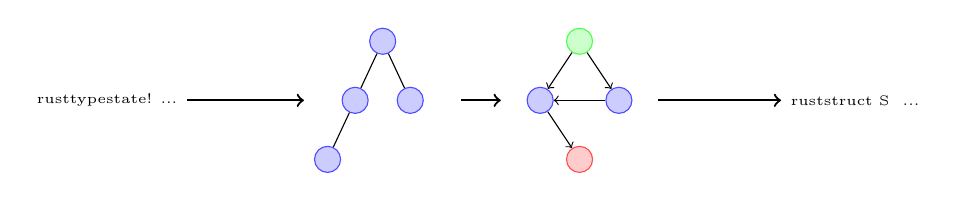
\begin{tikzpicture}
        \tikzstyle{code} = [fill=white, font=\tiny]

        \node[code] (code) at (0,0) {\tiny\mintinline{rust}{typestate!{ ... }}};

        \begin{scope}[shift={(3.5, 0.75)}]
            \tikzstyle{n}=[circle, draw=blue!70, fill=blue!20]
            \node[n] (root) at (0, 0) {};
            \node[n] (l1) at (-0.35, -0.75) {};
            \node[n] (l2) at (0.35, -0.75) {};
            \node[n] (l11) at (-0.7, -1.5) {};
            \draw[-] (root) -- (l1);
            \draw[-] (root) -- (l2);
            \draw[-] (l1) -- (l11);
        \end{scope}

        \begin{scope}[shift={(6, 0.75)}]
            \tikzstyle{n}=[circle, draw=blue!70, fill=blue!20]
            \tikzstyle{f}=[circle, draw=red!70, fill=red!20]
            \tikzstyle{s}=[circle, draw=green!70, fill=green!20]
            \node[s] (root) at (0, 0) {};
            \node[n] (l1) at (-0.5, -0.75) {};
            \node[n] (l2) at (0.5, -0.75) {};
            \node[f] (l11) at (0, -1.5) {};
            \draw[->] (root) -- (l1);
            \draw[->] (root) -- (l2);
            \draw[->] (l1) -- (l11);
            \draw[->] (l2) -- (l1);
        \end{scope}

        \node[code] (rust-code) at (9.5,0) {\mintinline{rust}{struct S { ... }}};

        \draw[->, thick] (code) -> (2.5, 0);
        \draw[->, thick] (4.5, 0) -> (5, 0);
        \draw[->, thick] (7, 0) -> (rust-code);

    \end{tikzpicture}
    \caption{
        From DSL specification to Rust code.
        First the DSL is parsed, then converted to a state machine and its properties checked
        (in the case some property is not respected, an error is issued).
        After the properties are validated, the Rust code is generated.
    }
    \label{fig:dsl-processing}
\end{figure}